\documentclass[12pt]{article}
\usepackage{a4wide}
\usepackage{graphicx}


\parindent 0pt
\parskip 6pt

\begin{document}

\thispagestyle{empty}

\rightline{\large Oliver Lane}
\medskip
\rightline{\large\ Trinity Hall}
\medskip
\rightline{\large\ ojgl2}

\vfil

\centerline{\large Part II Project Progress Report}
\vspace{0.4in}
\centerline{\Large\bf Audio Fingerprinting for Music Recognition}
\vspace{0.3in}
\centerline{\large 23rd January 2015}

\vfil

{\bf Name:} Oliver Lane (ojgl2@cam.ac.uk)

\vspace{0.2in}

{\bf Project Supervisor:} Vaiva Imbrasait\'{e}

\vspace{0.2in}

{\bf Director of Studies:} Professor Simon Moore

\vspace{0.2in}

{\bf Overseers:} Dr. Markus Kuhn and Dr. Neal Lathia

\vfil
\eject

\cleardoublepage
\setcounter{page}{1}

\section*{Achievements To Date}

Broadly, I have achieved almost everything that was outlined in the first 4 work packages in my original proposal.

I began by researching several different music recognition algorithms, focussing mostly on the two referenced in the proposal. I spent 2-3 weeks familiarising myself with MATLAB and MIRToolbox, which were the technologies I chose to use to implement my project. I also investigated how to use MATLAB to connect to a database, since all of the algorithms I looked at required one.

Once I was reasonably comfortable with the technologies, I drew up a basic system structure for the implementations, and began implementation of the two algorithms in my original proposal. The system structure is included below in Figure 1.

I began with the algorithm used by \emph{Shazam} and presented by Avery Li-Chun Wang in \emph{An Industrial-Strength Audio Search Algorithm}, which I had started by the end of Michaelmas term and finished implementing in the first two weeks of the Christmas break. This algorithm has a few parameters which aren't fully specified in the paper and may need some experimentation once I have tested it on more challenging test cases, in particular to do with its peak detection stage.

I used the rest of the break to fully implement the algorithm proposed in \emph{A Highly Robust Audio Fingerprinting System} by Jaap Haitsma and Ton Kalker. This algorithm was more concretely specified in the paper than the first algorithm was, so there is less to experiment with here.

The work over the Christmas break included some shared code for features such as reading audio from files and running a set of tests against an implementation.

Some basic testing has been carried out, using unmodified clips of songs in the library of lengths 3, 5 and 10 seconds. I have also started to create some more complex test cases including adding white noise to the unmodified clips at different levels.

\begin{figure}[htbp]
  \centering
  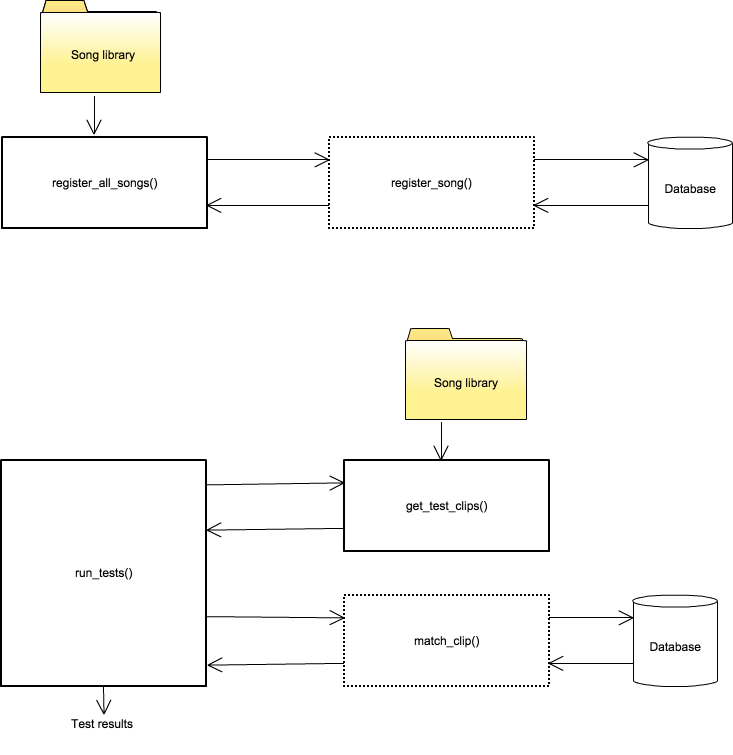
\includegraphics[width=\linewidth]{architecture}
  \caption{Structure of the system. Methods with dotted borders are algorithm-specific, and are swapped out to test different algorithms.}
\end{figure}


\newpage


\section*{Unexpected Difficulties and Changes}

Although I originally anticipated that MIRToolbox, a music information retrieval library, would be useful in the implementation of the algorithms, I found it to be difficult to use and not particularly useful anyway. It also has not been updated to work with the latest version of MATLAB. 

I found replacements for my two main planned uses of the library in the MATLAB Signal Processing Toolbox and an open source function called Fast 2D Peak Finder, respectively. In light of this, I decided not to use MIRToolbox.

Originally, I assumed that database integration with MATLAB would be trivial to set up, but I overlooked the fact that the standard solution for this is within a toolbox which isn't included under the university's license. 

Luckily, I found an alternative open source solution based on SQLite 3, which meant that I did not have to pay for the toolbox or find a way to obtain a license for it through the university. It's possible that a solution based on a more fully featured SQL implementation would speed my implementations up a little, but I deemed this unimportant since all of the algorithms I am comparing will use the SQLite implementation, and any speed improvements wouldn't be guaranteed anyway.

\section*{Timetable Evaluation}

I have mostly stuck to the timetable stated in my proposal, but I have made a couple of changes as I have progressed.

Firstly, it turned out to be easier to write the code which is shared between the implementations in parallel with the implementations themselves, since some subtleties didn't become apparent until I was writing the implementations. 

Secondly, I fell 1-2 weeks behind my schedule on writing my dissertation, and have decided to restructure this part of my plan based on a conversation with my Director of Studies and where I think I am at the moment in the project.

I now intend to write the preparation section first, followed by the introduction and conclusion, followed by the other sections. I hope that this will help me structure the dissertation better, and avoid some later restructuring and rewriting. 

Finally, although I have started work on my full set of test clips as outlined in work package 4 from the proposal, I have realised that the process of running and analysing the tests will inform the process of creating more clips, so I have pushed back delivery of the full set to work package 6 (due 1st March).

An updated timetable for the remainder of the project is included below. I don't see these changes as introducing any major added time pressure, since I structured the whole timetable to give me time at the end in case of setbacks and to make optional improvements.

I don't currently plan to implement a third algorithm for comparison, but this may change if one of the work packages takes significantly less time than anticipated.


\section*{New Timetable and Milestones}

\subsection*{Work package 5 (due 30th Jan)}
Write progress report and presentation.

\emph{Deliverables: Progress report and presentation}

\emph{Deadline (30th Jan): Progress report}

\subsection*{Work package 6 (due 1st Mar)}
Fully test the algorithms and produce diagrams to show the results. Write first drafts of the preparation, introduction and conclusion sections of the dissertation, and a first draft of the evaluation section. Finish the implementation section.

\emph{Deliverables: Results of thorough tests, and a full set of test clips. Drafts of preparation, introduction and conclusion sections. Finished implementation sections.}

\subsection*{Work package 7 (due Mar 15th)}
First draft of dissertation completed (to coincide with end of Lent term, so as to give time for my supervisor to give feedback and for me to concentrate mostly on revision over the Easter break).

\emph{Deliverables: First draft of full dissertation (previously completed drafts plus implementation and evaluation sections)}

\subsection*{Work package 8 (due May 7th)}
Keep the project ticking over, but exam preparation will take precedence at this point. Discuss dissertation with my supervisor, and review the whole project. Make any improvements possible in the time left.

Hand in final draft of dissertation. 

\emph{Deliverables: Final draft of dissertation}

\emph{Deadline (15th May): Dissertation}

\end{document}

